\chapter{Estudo de Caso }
% : Requisitos, Organização, Métodos, Design, Implementação e Testes
\label{cap:estudo_caso}
Este capítulo apresenta o contexto, os requisitos, a organização, os métodos, o design, a implementação e os testes realizados no desenvolvimento do estudo de caso em uma plataforma de notícias sobre tecnologia chamada WallTech.

\section{Contexto}
\label{section:contexto}
O estudo de caso é realizado em uma empresa fictícia chamada WallTech, uma plataforma de notícias sobre tecnologia que tem como objetivo fornecer conteúdos atualizados e relevantes sobre inovações e tendências do setor. Nela, os usuários podem acessar e buscar notícias utilizando palavras-chave, tanto em dispositivos móveis quanto em computadores, graças ao design responsivo da aplicação.  

Visando melhorar a experiência do usuário (UX) e otimizar o desempenho da plataforma, os gestores de tecnologia da WallTech decidiram realizar um estudo comparativo entre duas abordagens de renderização: \acrfull{csr} e \acrfull{ssr}. Para isso, optou-se pelo desenvolvimento de dois protótipos da plataforma, um com \acrshort{csr} utilizando React e outro com \acrshort{ssr} utilizando Next.js, com o objetivo de analisar qual modelo de renderização apresenta melhores resultados em termos de velocidade de carregamento, interatividade e no \english{\acrfull{seo}}.

A Figura \ref{fig:caso-uso-walltech} apresenta o diagrama de caso de uso da plataforma WallTech, mostrando as principais funcionalidades disponíveis para o usuário anônimo. O diagrama ilustra as interações do usuário com o sistema, permitindo que ele visualize a lista de notícias mais recentes, acesse os detalhes de uma notícia ao clicar nela, ou realize buscas específicas utilizando palavras-chave.  

\begin{figure}[H]
  \centering
  \caption{Diagrama de caso de uso}
  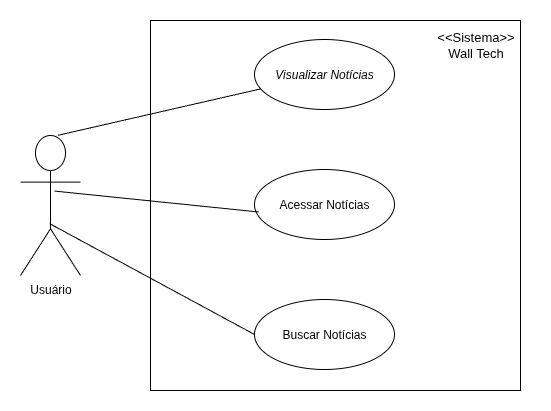
\includegraphics[width=0.7\textwidth]{media/wall_tech_use_case.png}
  \legend{Fonte: os autores.}
  \label{fig:caso-uso-walltech}
\end{figure}



\section{Processo de Desenvolvimento}
\label{section:processo-desenvolvimento}
O processo de desenvolvimento utilizado para construir a plataforma WallTech segue a metodologia ágil \english{Kanban}. Essa metodologia de desenvolvimento ágil é baseada em um quadro de tarefas, no qual cada tarefa é representada por um cartão \cite{gomes2014kanban}. O quadro Kanban é dividido em colunas que representam o estado atual de cada tarefa. As colunas mais comuns são: \english{To Do}, \english{In Progress} e \english{Done}, e o quadro é atualizado conforme as tarefas são realizadas. Além dessas colunas, o processo foi adaptado para incluir colunas adicionais como \english{Docs} e \english{Test}, permitindo que a documentação e os testes fossem gerenciados de forma organizada e eficiente durante o desenvolvimento.

A Figura \ref{fig:kanban-walltech} apresenta um exemplo do quadro Kanban utilizado no \english{GitHub Projects}, mostrando a organização das tarefas e o progresso do desenvolvimento da plataforma WallTech. O quadro reflete a estrutura de colunas adaptada, proporcionando uma visão clara do fluxo de trabalho da equipe, o que facilita o acompanhamento das tarefas em diferentes estágios.

Após a definição das funcionalidades principais do sistema, as tarefas foram inicialmente documentadas como \english{user stories}. As \english{user stories} são descrições simples e compreensíveis das funcionalidades a serem implementadas, permitindo uma comunicação clara entre a equipe de desenvolvimento e as partes interessadas. Cada \english{user story} é associada a um conjunto de requisitos específicos e uma definição de pronto, facilitando a compreensão do que precisa ser desenvolvido.

A partir dessas \english{user stories}, as \english{issues} foram criadas no \english{GitHub Projects}. Cada \english{issue} representa uma tarefa específica que deve ser realizada, baseada nas \english{user stories}. No \english{GitHub Projects}, essas \english{issues} são organizadas nas colunas do quadro Kanban, permitindo que a equipe visualize o progresso de cada tarefa e as mova conforme o andamento do trabalho.

A Figura \ref{fig:kanban-userstories} mostra um exemplo de cartão \english{issue} no \english{GitHub Projects}, ilustrando como as \english{user stories} são transformadas em tarefas e organizadas dentro do quadro Kanban. Cada \english{issue} possui detalhes sobre a tarefa, como descrições, prioridade e prazo, facilitando o gerenciamento e a execução das atividades no time de desenvolvimento.

\begin{figure}[H]
  \centering
  \caption{Exemplo de quadro Kanban no \english{GitHub Projects}}
  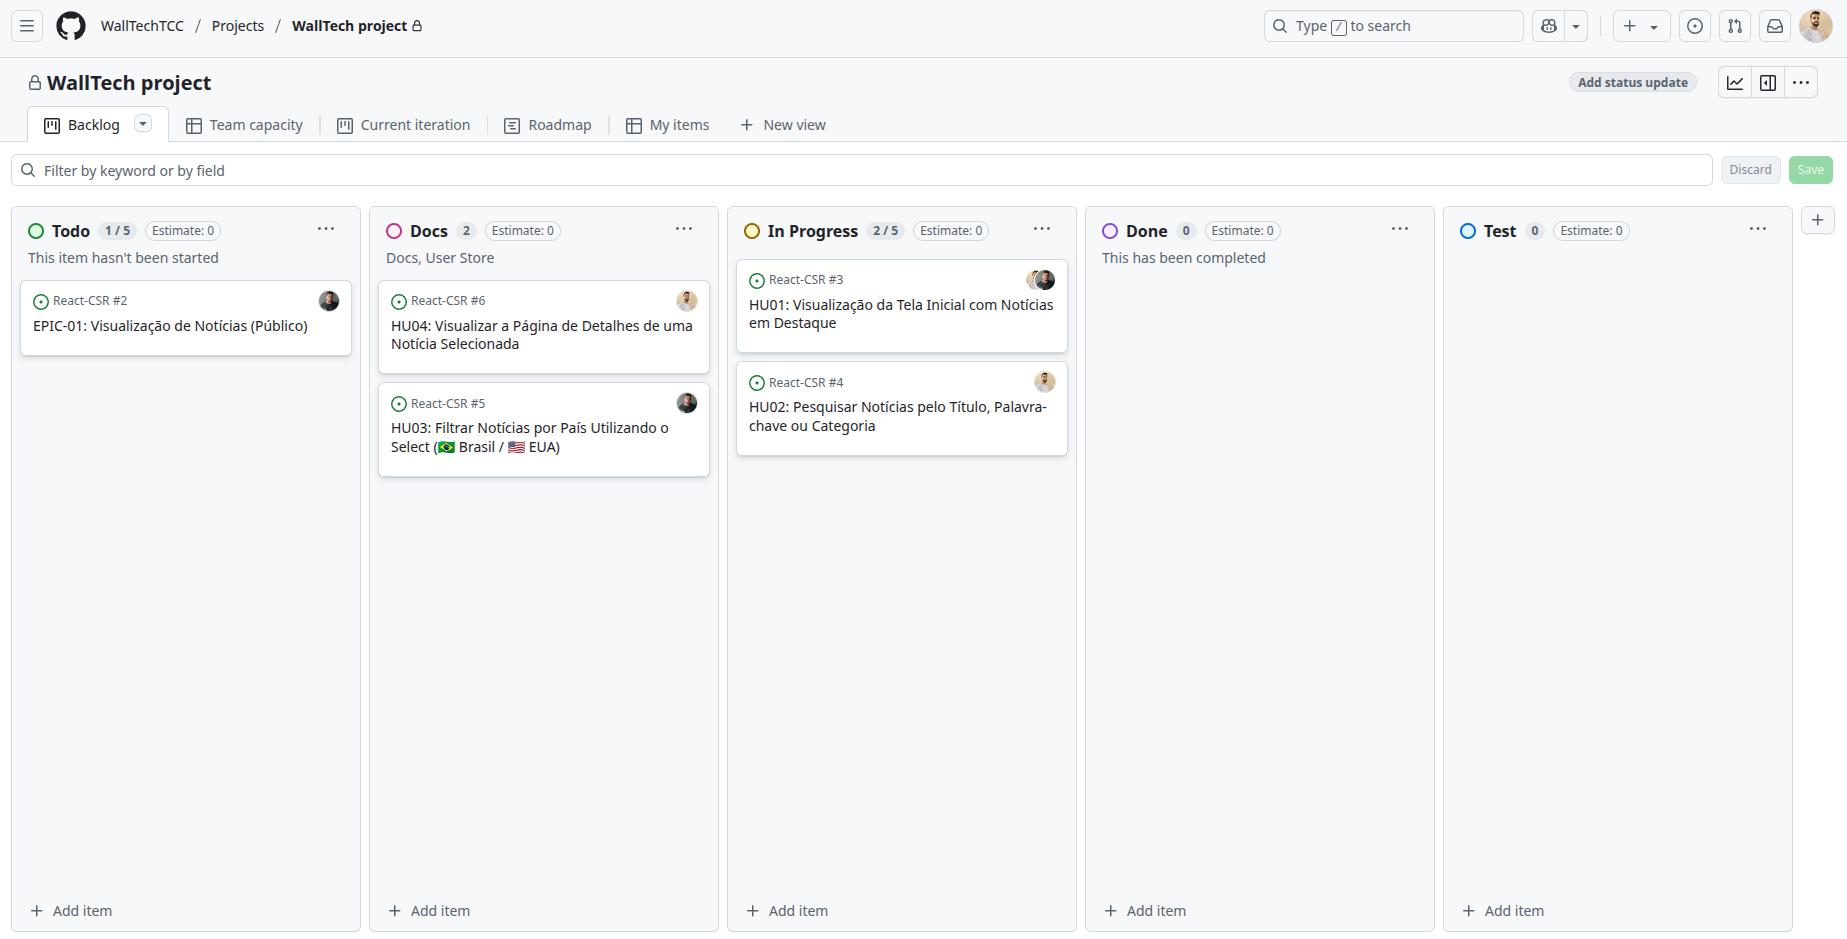
\includegraphics[width=1.0\textwidth]{media/wall_tech_kanban.png}
  \legend{Fonte: os autores.}
  \label{fig:kanban-walltech}
\end{figure}

\begin{figure}[H]
  \centering
  \caption{Exemplo de cartão \english{issue} no \english{GitHub Projects}}
  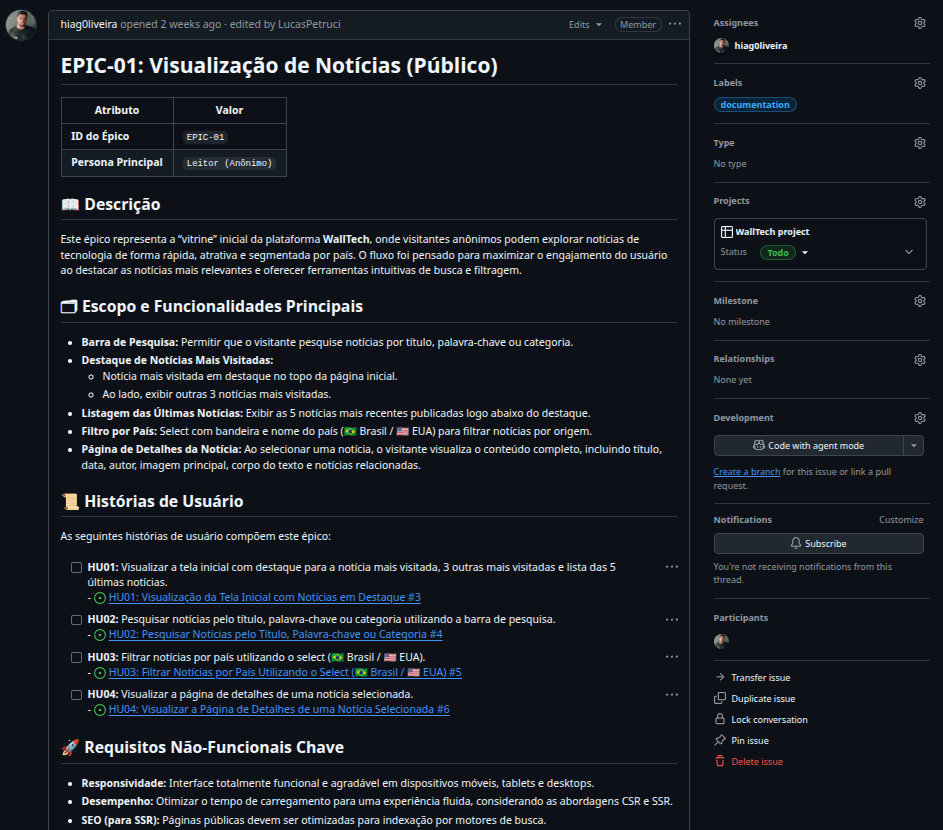
\includegraphics[width=0.7\textwidth]{media/wall_tech_epic.png}
  \legend{Fonte: os autores.}
  \label{fig:kanban-userstories}
\end{figure}

\section{Requisitos}
\label{section:requisitos}
Os requisitos do sistema foram definidos com base nas necessidades dos usuários e nas funcionalidades desejadas para a plataforma WallTech. A seguir, são apresentados os principais requisitos funcionais e não funcionais identificados para o desenvolvimento da aplicação.

\subsection{Requisitos Funcionais}
\label{subsec:requisitos-funcionais}
A Figura \ref{fig:sequence-diagram} ilustra um diagrama de sequência da plataforma WallTech, onde o usuário pode visualizar notícias e navegar para os detalhes de uma notícia específica.

No diagrama, o processo começa quando o usuário acessa o site da WallTech, e o navegador faz a requisição para carregar a página inicial. O servidor Next.js então busca as notícias padrão, como as mais recentes e em destaque, na API Externa (NewsAPI). O servidor renderiza a página HTML completa e a envia ao navegador para exibição, permitindo que o usuário veja as notícias em português.


\begin{figure}[H]
  \centering
  \caption{Diagrama de sequência da plataforma WallTech}
  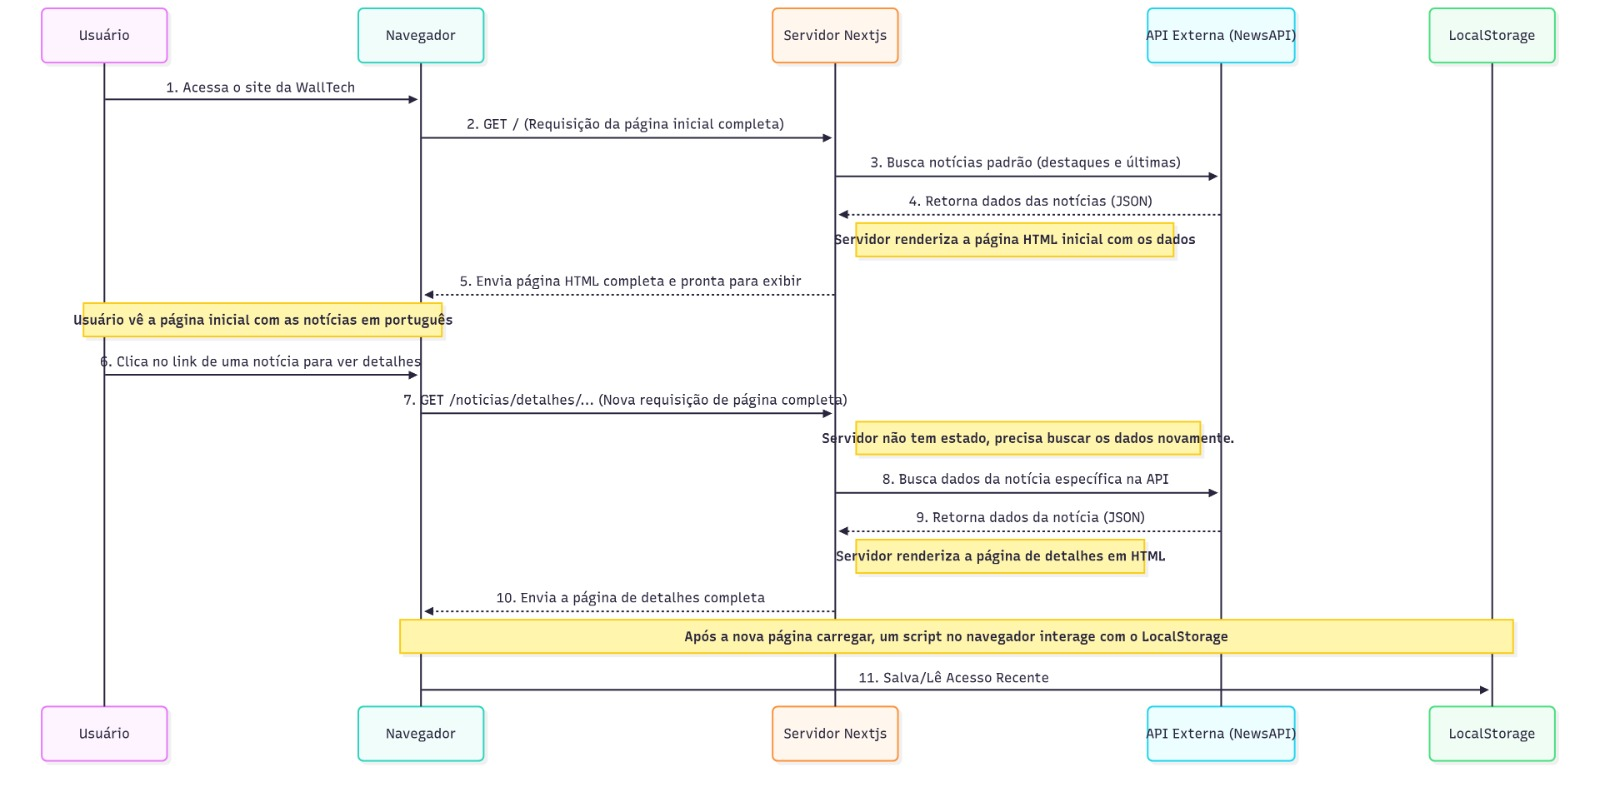
\includegraphics[width=0.7\textwidth]{media/wall_tech_sequence_diagram.jpeg}
  \legend{Fonte: os autores.}
  \label{fig:sequence-diagram}
\end{figure}


\section{Design do Sistema}
\label{cap:design}

O design do sistema foi orientado para refletir as diferenças estruturais entre as abordagens \acrshort{spa} e \acrshort{mpa}, levando em consideração os requisitos funcionais da plataforma \textit{WallTech}. Esta vitrine digital exibe notícias de tecnologia obtidas por meio da \textit{NewsAPI}, com recursos de busca, filtragem e destaque de conteúdo segmentado por país. Não há backend próprio, sendo todas as chamadas feitas diretamente para a API externa, o que simplifica a arquitetura e acentua o papel do frontend na renderização de conteúdo.

Para modelagem arquitetural e comportamental, foram utilizados diagramas da UML, incluindo:
\begin{itemize}
  \item \textbf{Diagrama de Caso de Uso}, para representar as principais funcionalidades acessadas pelos usuários visitantes.
  \item \textbf{Diagrama de Sequência}, a fim de ilustrar o fluxo de interação entre navegador e a \textit{NewsAPI} durante operações como busca e carregamento de notícias.
  \item \textbf{Diagrama de Componentes}, para representar os módulos da aplicação, como a interface, o serviço de requisição à API, e os componentes de renderização.
\end{itemize}

As decisões de design foram fundamentadas em boas práticas para renderização web discutidas por \cite{osmani2025}, bem como nas diretrizes da literatura especializada em arquitetura de frontend, como apresentado pela \cite{atori2024}.

Segundo \cite{osmani2025}, a escolha entre renderização no cliente ou no servidor deve considerar o contexto da aplicação, os requisitos de desempenho e os objetivos de SEO. Já o artigo da \cite{atori2024} destaca que SPAs tendem a oferecer maior fluidez e interatividade, enquanto MPAs são mais eficazes em aplicações que dependem de indexação e acessibilidade.

\subsection{Arquitetura SPA}

A versão \acrshort{spa} da aplicação foi projetada com foco em responsividade e fluidez de interação. Utilizando bibliotecas como React, a renderização do conteúdo é feita inteiramente no navegador, após o carregamento inicial de um documento \texttt{HTML} mínimo. Todas as requisições são feitas dinamicamente via \texttt{fetch} para a \textit{NewsAPI}, permitindo uma experiência de uso imersiva sem recarregamentos completos de página.

Essa abordagem reduz a carga no servidor, melhora a experiência de usuário em conexões rápidas e facilita a manutenção do código por meio de componentes reutilizáveis. Por outro lado, apresenta desafios quanto à indexação por mecanismos de busca, dado que o conteúdo depende da execução de JavaScript, conforme destacado por \cite{osmani2025}. Essa limitação pode ser parcialmente mitigada com técnicas como \textit{pre-rendering} e \textit{hydration} progressiva.

O diagrama de componentes da SPA evidencia a centralização da lógica no navegador, enquanto o diagrama de sequência demonstra o ciclo de vida de requisições e renderização client-side.

\subsection{Arquitetura MPA}

A versão \acrshort{mpa}, por sua vez, simula a renderização \acrshort{ssr}, em que cada rota representa uma nova página entregue já montada. Neste modelo, cada requisição à aplicação resulta na obtenção de uma nova instância de HTML contendo os dados pré-processados. Frameworks como Next.js permitem implementar essa estratégia, mesmo quando os dados provêm de APIs externas como a \textit{NewsAPI}.

Esse tipo de renderização favorece o desempenho inicial (menor \acrshort{fcp}) e melhora a indexação do conteúdo pelos mecanismos de busca, como discutido pela \cite{atori2024}. Na aplicação, isso se traduz em páginas com conteúdo estático inicial pronto para rastreamento, mesmo que a interatividade seja ativada posteriormente via JavaScript (\textit{hydration}).

O diagrama de componentes da MPA demonstra a responsabilidade do servidor em montar o HTML completo, enquanto o diagrama de sequência mostra o papel da API externa na geração do conteúdo antes da entrega ao navegador.



\section{Implementação}
\label{sec:implementacao}

Esta seção descreve o conjunto de tecnologias, bibliotecas e ferramentas que são empregadas para a construção das duas versões do sistema de prova de conceito, detalhando a fundamentação para a escolha de cada componente do ecossistema de desenvolvimento. O gerenciamento do código-fonte e do ciclo de vida do projeto é realizado com o sistema de controle de versão \textbf{Git} e a plataforma de hospedagem \textbf{GitHub}, conforme as práticas descritas na Seção~\ref{sec:git-github}.

Ambas as implementações consomem dados da mesma fonte externa, a \textbf{News API}, uma \acrshort{api} RESTful que fornece o conteúdo jornalístico para a aplicação, como detalhado na Seção~\ref{sec:news-api}. Para garantir a consistência visual e a qualidade da interface entre as duas arquiteturas, utiliza-se a biblioteca de componentes \textbf{shadcn/ui}, que oferece um conjunto de componentes acessíveis e personalizáveis, conforme apresentado na Seção~\ref{sec:ferramentas-modernas}.

\subsection{Implementação da Aplicação SPA}
\label{ssec:implementacao_spa}

A implementação da \acrfull{spa} é desenvolvida utilizando a biblioteca \textbf{React} na sua versão 18. O React é uma biblioteca JavaScript declarativa, mantida pela Meta, focada na construção de interfaces de usuário a partir de componentes reutilizáveis. Sua adoção neste projeto se dá por sua vasta popularidade no mercado e ao seu paradigma de componentização, que facilita a criação de UIs modulares e de fácil manutenção \cite{react2025}. A eficiência da renderização é otimizada pelo uso de um DOM Virtual, um conceito central da biblioteca que minimiza as manipulações diretas no navegador.

Para a estruturação inicial do projeto e o gerenciamento do ambiente de desenvolvimento, utiliza-se a ferramenta de \textit{build} \textbf{Vite}. O Vite é um ecossistema de desenvolvimento frontend moderno que oferece um servidor de desenvolvimento com recarregamento rápido (\textit{Hot Module Replacement}) e um processo de compilação (\textit{build}) otimizado, que resulta em pacotes de produção menores e mais eficientes \cite{vite_docs}.

O roteamento no lado do cliente, uma característica fundamental da arquitetura SPA, implementa-se com a biblioteca \textbf{React Router}. Trata-se da solução padrão para navegação em aplicações React, que possibilita a criação de uma experiência de usuário fluida e sem recarregamentos de página ao manipular a \acrshort{api} de Histórico do navegador \cite{react_router_docs}. A comunicação com a News API é realizada por meio da \acrshort{api} \texttt{fetch}, nativa dos navegadores modernos.

\subsection{Implementação da Aplicação MPA}
\label{ssec:implementacao_mpa}

A implementação da \acrfull{mpa}, com foco em \acrfull{ssr}, é desenvolvida com o \emph{framework} \textbf{Next.js} na versão 14. O Next.js é um meta-framework baseado em React, mantido pela Vercel, que se posiciona como uma solução completa para a construção de aplicações web de produção. Sua escolha para este estudo de caso justifica-se por ser a principal referência de mercado para a implementação de \acrshort{ssr} no ecossistema React, oferecendo uma estrutura robusta e opinativa \cite{nextjs2024}.

O \emph{framework} opera sobre um ambiente \textbf{Node.js}, o que permite a execução de código JavaScript no lado do servidor \cite{nodejs2025}. Essa capacidade é a base da renderização no servidor, onde o Next.js utiliza funções específicas, como a \texttt{getServerSideProps}, para buscar dados de fontes externas e pré-renderizar o HTML completo de uma página antes de enviá-la ao navegador. Além disso, o Next.js implementa um sistema de roteamento baseado no sistema de arquivos, onde a estrutura de diretórios da pasta \texttt{pages} define automaticamente as rotas da aplicação, simplificando a configuração e a manutenção do projeto.